\documentclass[screen, aspectratio=169]{beamer}
\usepackage[T1]{fontenc}
\usepackage[utf8]{inputenc}

% Use the NTNU-temaet for beamer 
% \usetheme[style=ntnu|simple|vertical|horizontal, 
%     language=bm|nn|en, 
%     smalltitle, 
%     city=all|trondheim|alesund|gjovik]{ntnu2017}
\usetheme[style=ntnu,language=en]{ntnu2017}

\usepackage[english]{babel}
\usepackage[style=numeric,backend=biber,natbib=false,sorting=none]{biblatex}

\title[HCI-intro]{Human Computer Interaction}
\subtitle{Design \& Evaluation in HCI}
\author[A. Xamb{\'o}]{Anna Xamb{\'o}}
\institute[NTNU]{Department of Music, NTNU}
\date{24 October 2019}
%\date{} % To have an empty date

\addbibresource{../hci-lectures.bib} % Add bibliography database

% Set the reference style to numeric.
% See here: http://tex.stackexchange.com/questions/68080/beamer-bibliography-icon
\setbeamertemplate{bibliography item}[text] 

% Set bibliography fonts to a small size.
\renewcommand*{\bibfont}{\footnotesize}

\begin{document}

\begin{frame}
  \titlepage
\end{frame}

% Alternatively, special title page command to get a different background
% \ntnutitlepage

\begin{frame}
\frametitle{Learning Outcomes}
\begin{itemize}
\item Identify key literature in HCI design and ergonomics.
\item Understand the trends in the approach to evaluation in the CHI conference / HCI discipline.
\item Establish connections between quantitative, qualitative and mixed research methods applied to HCI.
%\item Establish connections between quantitative, qualitative and mixed research methods from HCI applied to interactive music systems.
\item Conceptualize an approach to evaluation of a self-built musical instrument based on human-centered design.
\item Analyze the research methods and evaluation elements in a successful CHI paper submission.
\end{itemize}
\end{frame}
%
\begin{frame}
\frametitle{Preparation: Reading}
\begin{itemize}
\item Send a summary (1 page max.) of the following article:
\begin{itemize}
\item From Mice to Men - 24 years of Evaluation in CHI~\cite{Barkhuus.Rode.2007.evalchi}\\
\url{http://barkhu.us/barkhuus-altchi2007.pdf} 
\end{itemize}
The summary should include: the main topic of the paper, the approach used, the main findings, and the main contributions.
\end{itemize}
\end{frame}
%
\begin{frame}
\frametitle{Class Structure}
\begin{itemize}
\item 10.15-10.30 Warm-up activity, HCI design \& ergonomics.
\item 10.30-10.45 Research methods in HCI.
\item 10.45-11.00 Group discussion about the prep. reading.
%\item 11.00-11.15 Examples HCI evaluation in interactive music systems.
\item 11.00-11.15 Human-centered design.
\item 11.15-11.30 Team working: (1) What is your research question? (2) How to evaluate your prototype borrowing HCI methods? (3) What makes a good CHI paper?
\item 11.30-12.00 Final group discussion \& closing.
\end{itemize}
\end{frame}
%
\begin{frame}
\frametitle{Warm-up Activity}
TODO: Similarities / differences between the papers
 \begin{figure}
	
\includegraphics[scale=0.28]{img/mindmap-selected-papers.png}
    \end{figure}
\end{frame}
%
\begin{frame}
\frametitle{}
\Huge{HCI Design \& Ergonomics}
\end{frame}
%
\begin{frame}
\frametitle{The Design of Everyday Things}
 \begin{figure}
	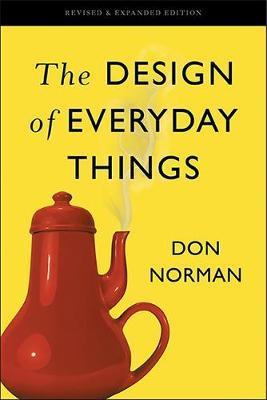
\includegraphics[scale=0.35]{img/Donald-Norman-The-Design-of-Everyday-Things.jpg}
    \end{figure}
    Norman, D. A. (2013/1988). \emph{The Design of Everyday Things}. Basic books. \cite{Norman.1988.psychology}
\end{frame}
%
\begin{frame}
\frametitle{The Design of Everyday Things}
 \begin{figure}
	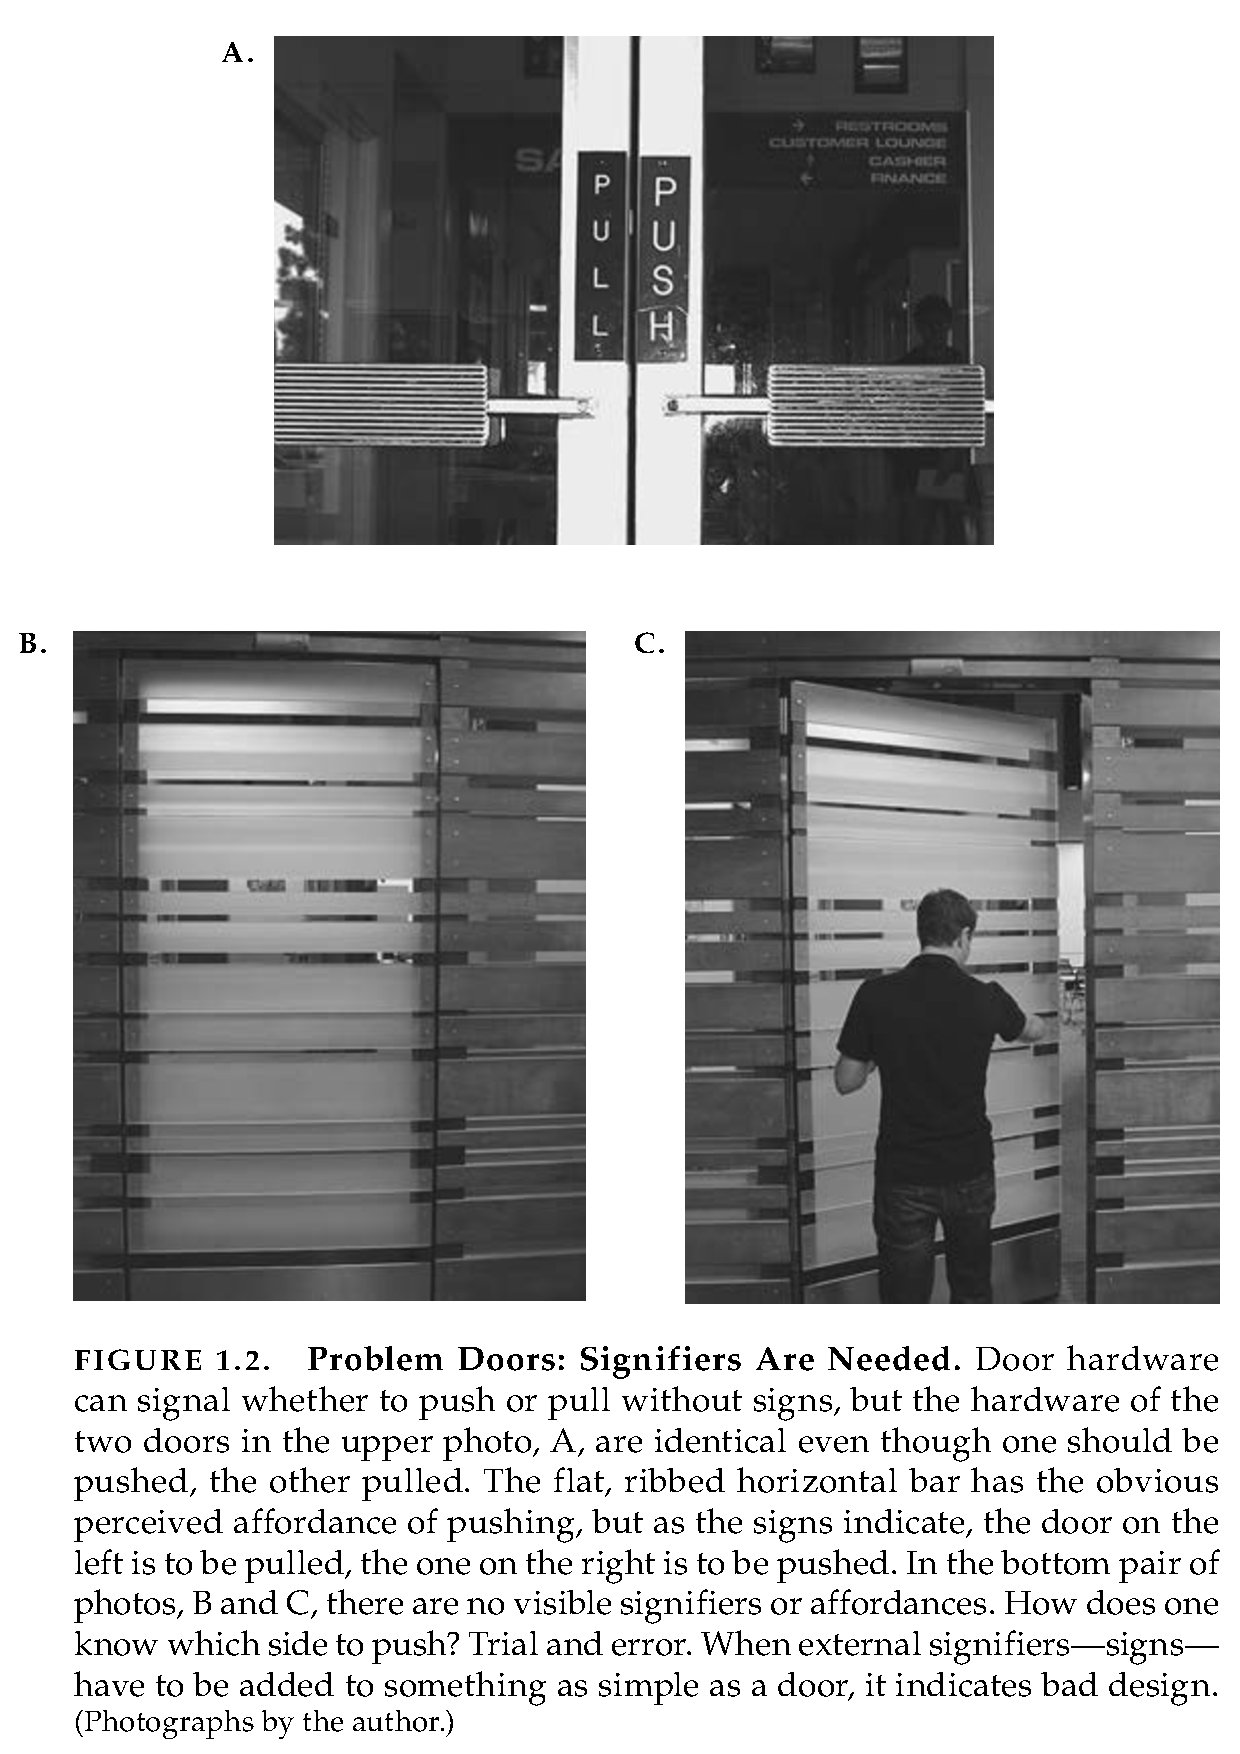
\includegraphics[scale=0.23]{img/Donald-Norman-doors.pdf}
    \end{figure}
\end{frame}
%
\begin{frame}
\frametitle{The Design of Everyday Things}
\begin{itemize}
\item \emph{Rules}: Make things visible, exploit natural relationships that couple function and control, and make intelligent use of constraints. 
\item \emph{Goal}: Guide the user effortlessly to the right action on the right control at the right time. 
\end{itemize}
\end{frame}
%
\begin{frame}
\frametitle{Emotional Design: Why We Love (or Hate) Everyday Things}
 \begin{figure}
	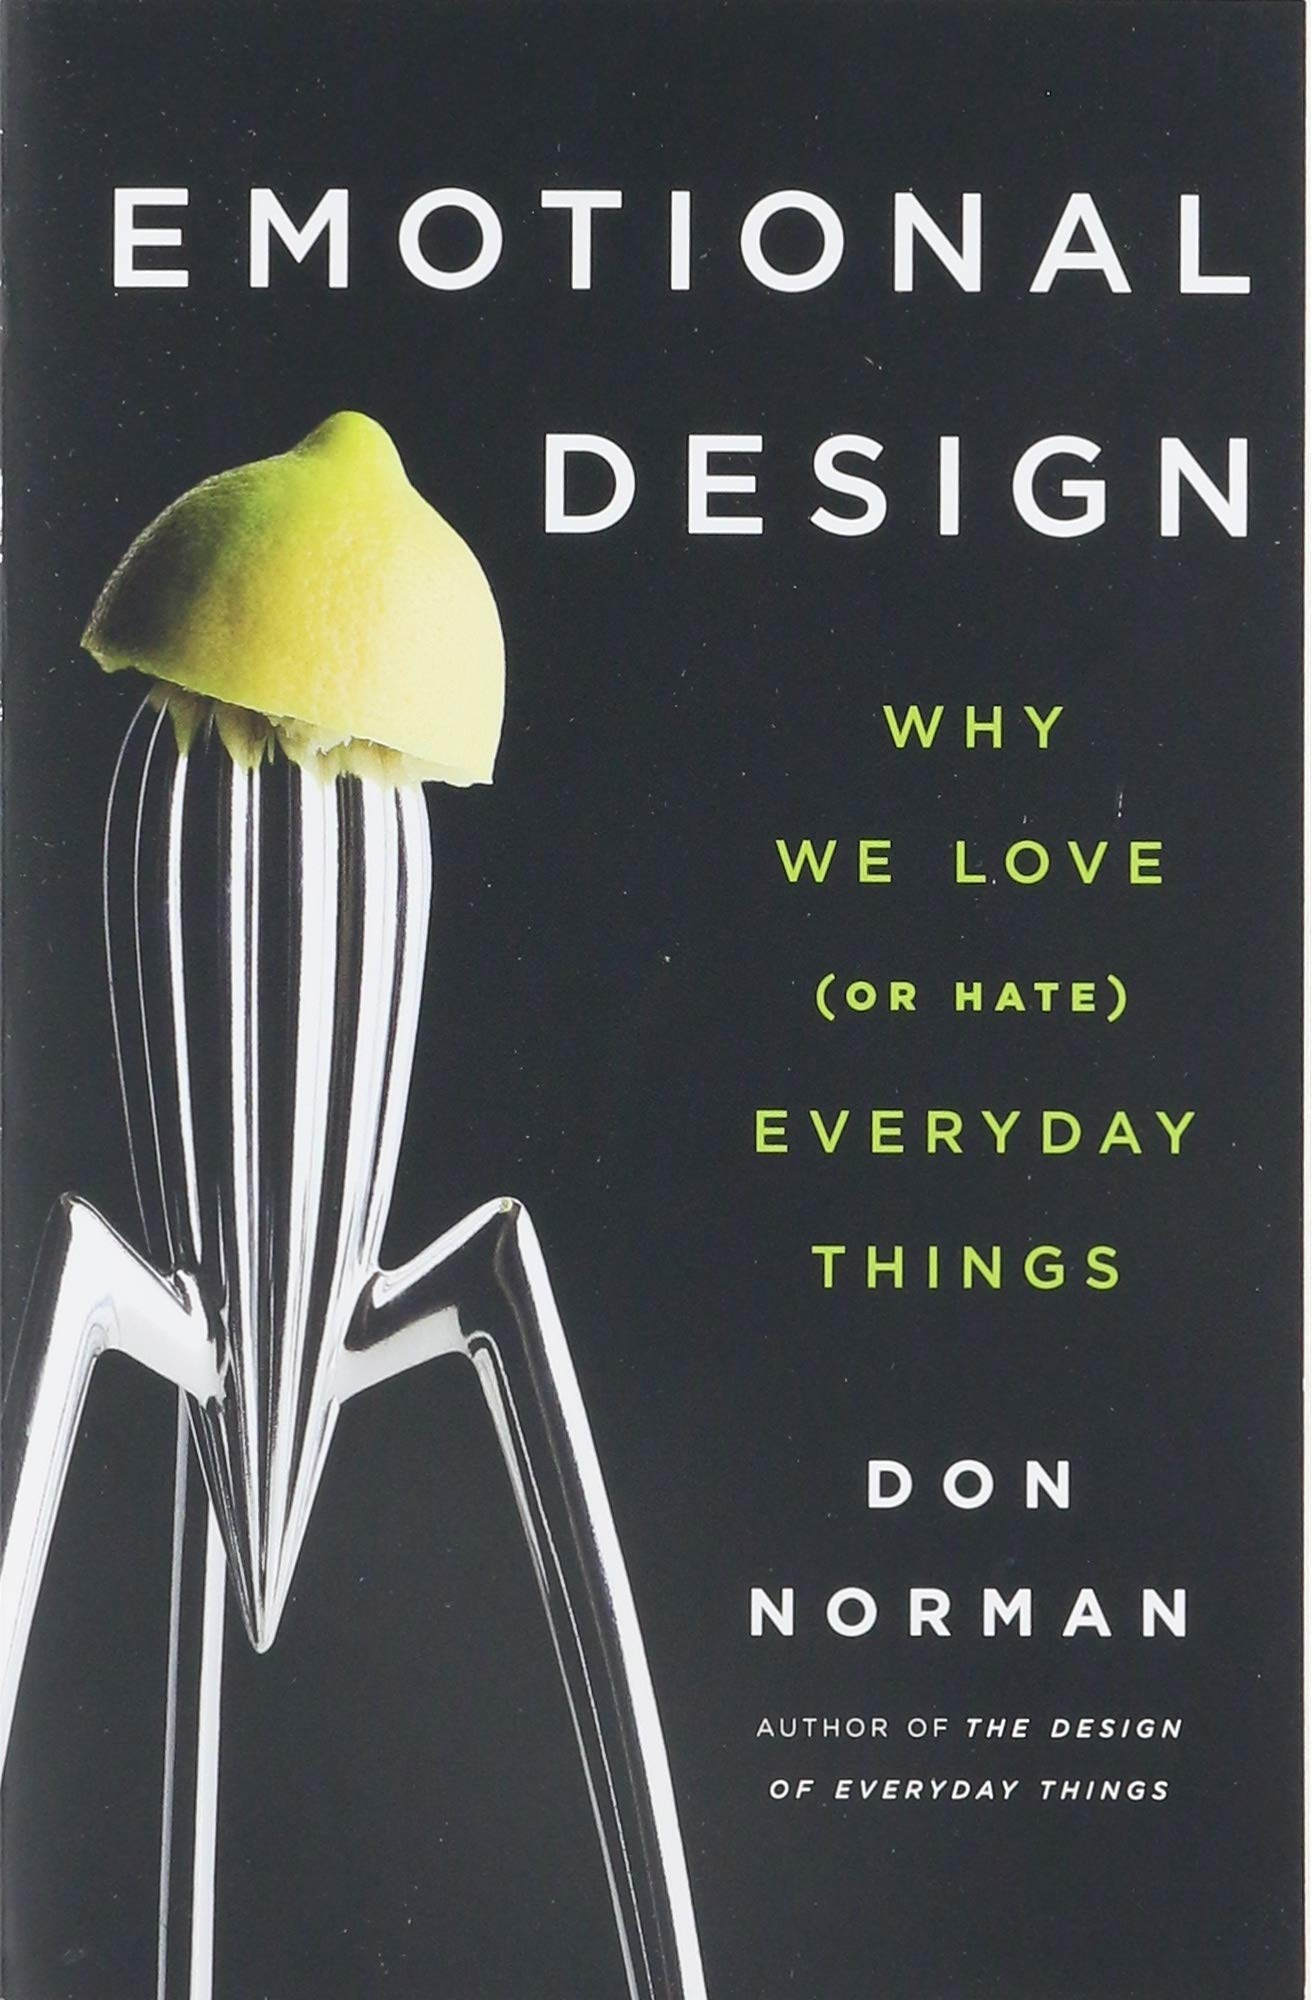
\includegraphics[scale=0.08]{img/Donald-Norman-Emotional-Design.jpg}
    \end{figure}
    Norman, D. A. (2004). \emph{Emotional Design: Why We Love (or Hate) Everyday Things}. Basic Civitas Books. \cite{Norman.2004.Emotional}
\end{frame}
%
\begin{frame}
\frametitle{Emotional Design: Why We Love (or Hate) Everyday Things}
 \begin{figure}
	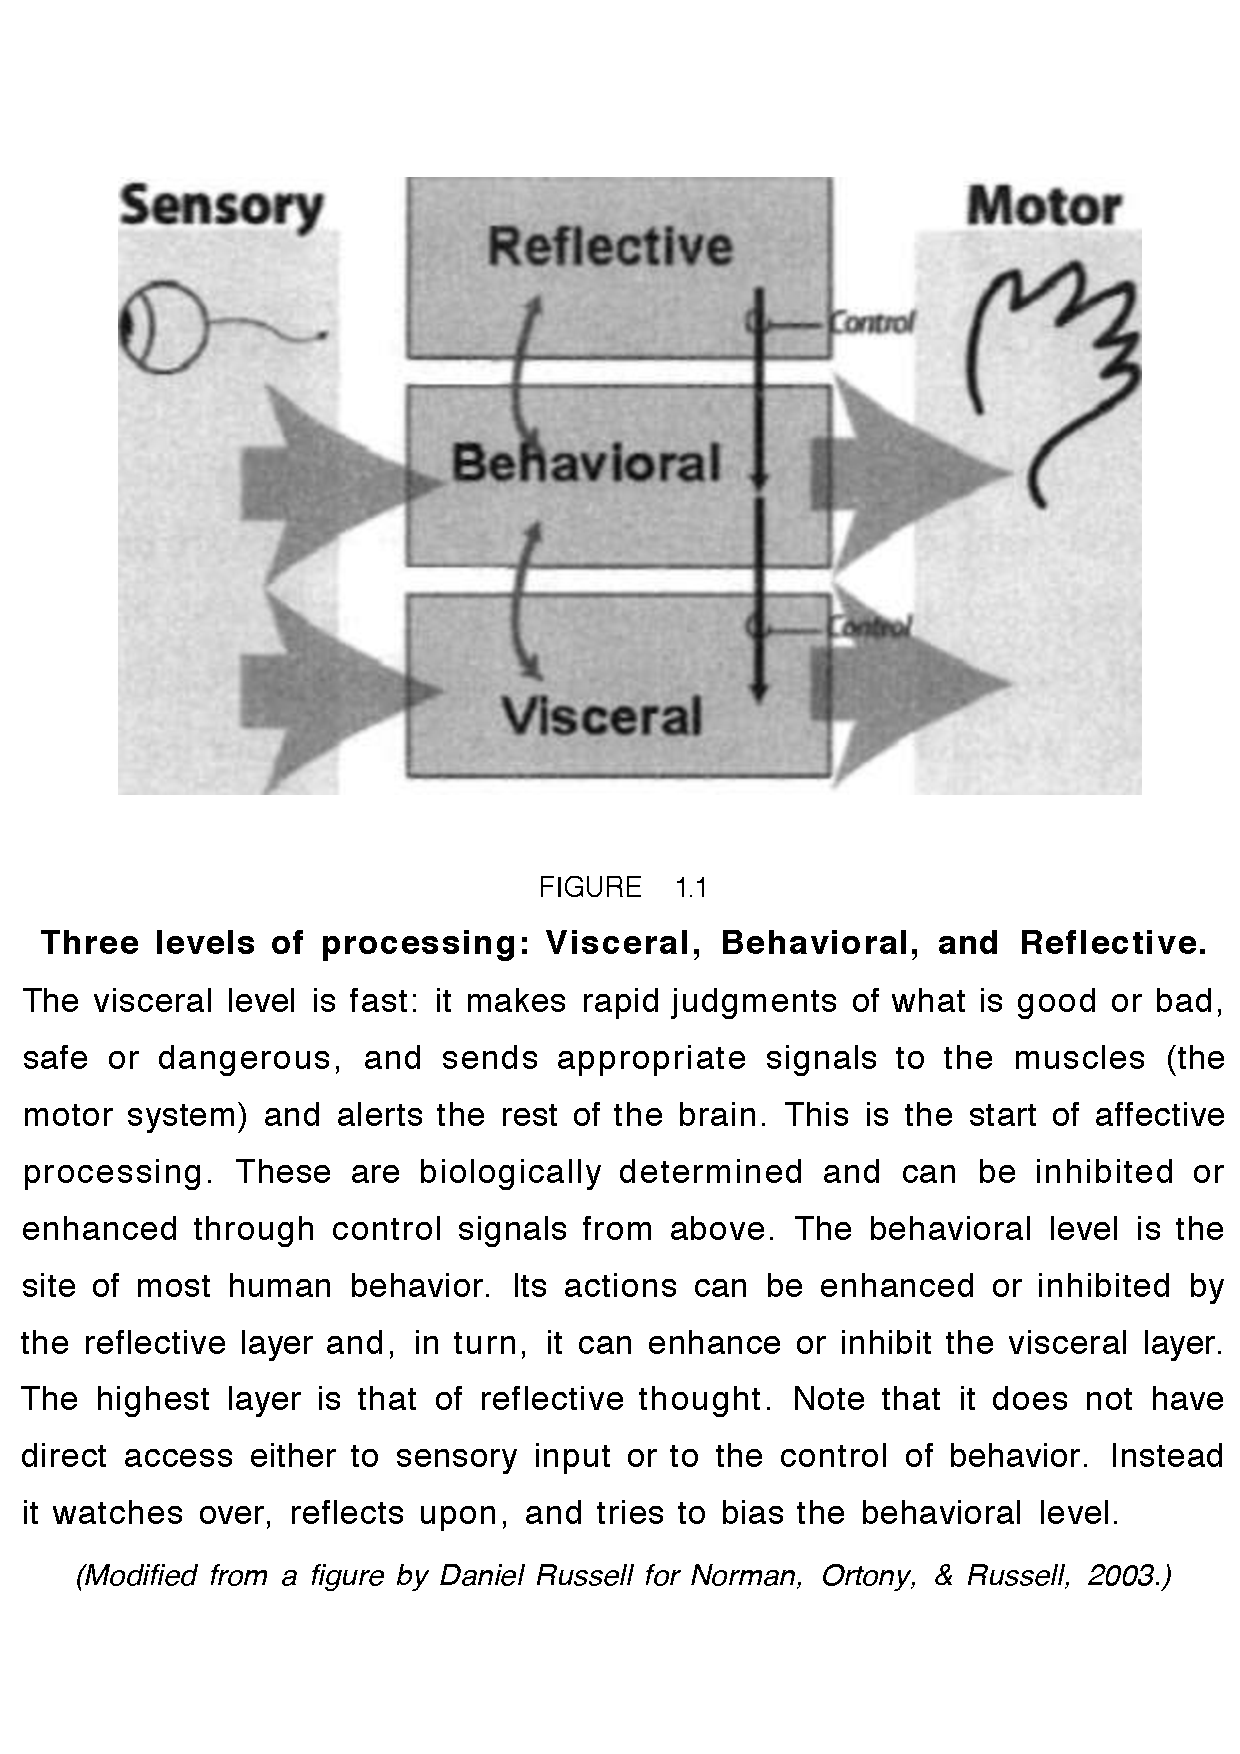
\includegraphics[scale=0.23]{img/Donald-Norman-3-levels-design.pdf}
    \end{figure}
\end{frame}
%
\begin{frame}
\frametitle{Emotional Design: Why We Love (or Hate) Everyday Things}
The three levels of processing can be mapped to product characteristics \cite[p.39]{Norman.2004.Emotional}
\begin{itemize}
\item \emph{Visceral design}: Appearance, form with powerful emotional signs (e.g. children's toys, clothes, furniture)
\item \emph{Behavioral design}: The pleasure of effectiveness of use, emphasis on the use of objects, performance and function matter (e.g. a shower)
\item \emph{Reflective design}: Self-image, personal satisfaction, memories, it is about message and culture and the meaning of the product or its use, prestige, perceived rarity and exclusiveness (e.g. a souvenir monument, a smartwatch)
\end{itemize}
\end{frame}
%
\begin{frame}
\frametitle{Emotional Design: Why We Love (or Hate) Everyday Things}
 \begin{figure}
	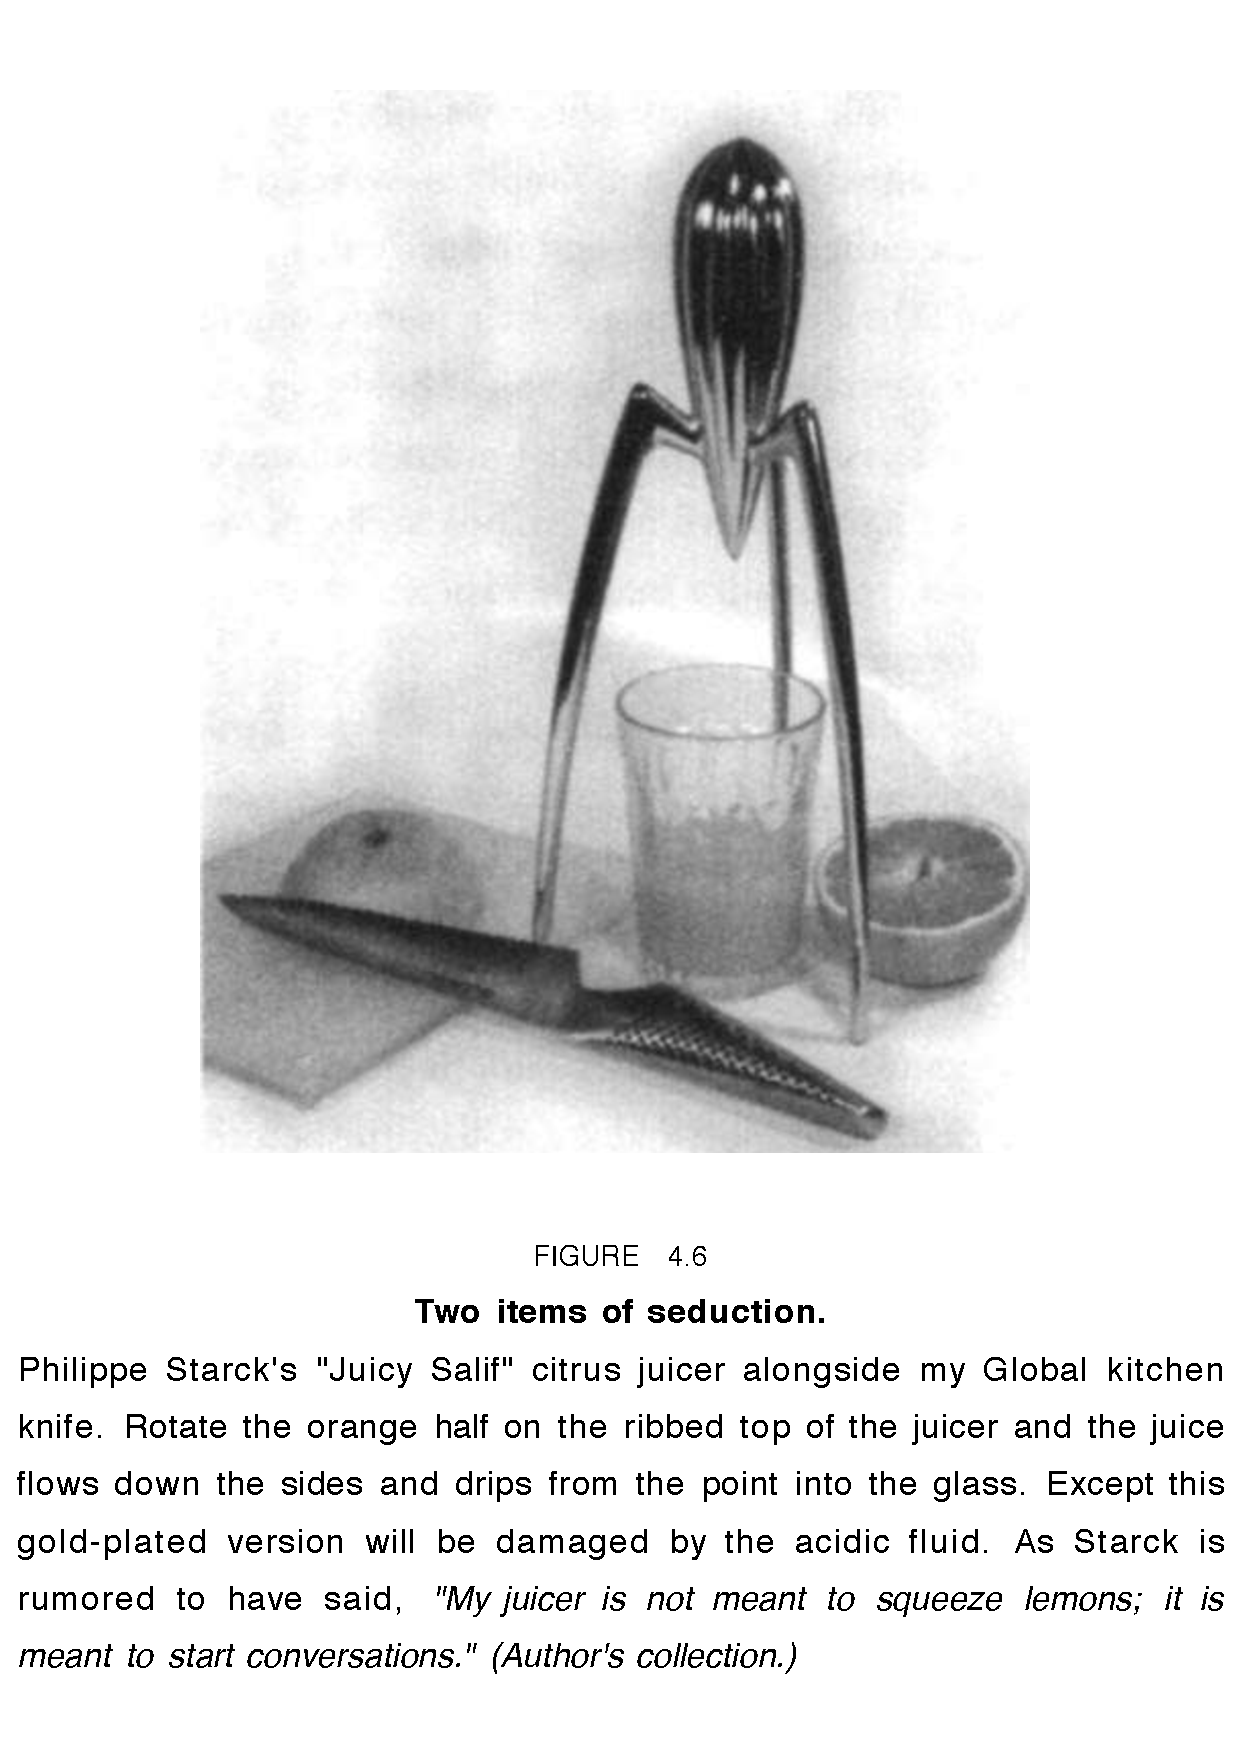
\includegraphics[scale=0.23]{img/Donald-Norman-juicer.pdf}
    \end{figure}
\end{frame}
%
\begin{frame}
\frametitle{Emotional Design: Why We Love (or Hate) Everyday Things}
Characteristics of Philippe Starck's Juicy Salif:
\begin{itemize}
\item Entices by diverting attention.
\item Delivers surprising novelty.
\item Goes beyond obvious needs and expectations.
\item Creates an instinctive response.
\item Espouses values or connections to personal goals.
\item Promises to fulfill these goals.
\item Lends the casual viewer to discover something deeper about the juicing experience.
\item Fulfills these promises.
\end{itemize} 
\end{frame}
%
\begin{frame}
\frametitle{Apple Human Interface Guidelines: Accessibility \& Inclusive Design\\Impairments and Accommodations}
 \begin{figure}
	
\includegraphics[scale=0.18]{img/apple-accessibility-icon_2x.png}
    \end{figure}
\begin{itemize}
\item Approximately one in seven people worldwide have a disability or impairment that affects the way they interact with the world and their devices. People can experience impairments at any age, for any duration, and at varying levels of severity. Situational impairments---temporary conditions such as driving a car, hiking on a bright day, or studying in a quiet library---can affect the way almost everyone interacts with their devices at various times.
\end{itemize} 
{\scriptsize \url{https://developer.apple.com/design/human-interface-guidelines/accessibility/overview/introduction/}    }
\end{frame}
%
%
\begin{frame}
\frametitle{Apple Human Interface Guidelines: Accessibility \& Inclusive Design\\Impairments and Accommodations}
 \begin{figure}
	
\includegraphics[scale=0.18]{img/apple-accessibility-icon_2x.png}
    \end{figure}
\begin{itemize}
\item Begin designing your app to be inclusive and accessible to everyone by reviewing the four main categories of impairments and the accessibility features that address them: \emph{Vision}, \emph{Hearing}, \emph{Physical and Motor}, \emph{Literacy and Learning}
\end{itemize} 
{\scriptsize \url{https://developer.apple.com/design/human-interface-guidelines/accessibility/overview/introduction/}    }
\end{frame}
%
\begin{frame}
\frametitle{Handbook of Human Factors and Ergonomics}
 \begin{figure}
	
\includegraphics[scale=0.3]{img/Salvendy-Handbook-Human-Factors-Ergonomics.jpg}
    \end{figure}
    Salvendy, G. (Ed.). (2012). Handbook of Human Factors and Ergonomics. John Wiley \& Sons. \cite{Salvendy.2012.handbook}\\
    Table of contents: \url{https://onlinelibrary.wiley.com/doi/book/10.1002/9781118131350}
\end{frame}
%
\begin{frame}
\frametitle{}
\Huge{Research Methods in HCI}
\end{frame}
%
\begin{frame}
\frametitle{Research Methods in HCI}
\begin{quote}
Choosing which method to use is a highly context-dependent issue related to a variety of factors including the primary purpose of the study, time constraints, funding, the participant pool, and the researchers' experience. \cite[p.25]{Lazar.et.al.2017.research}
\vspace{5mm}
Lazar, J., Feng, J. H. and Hochheiser, H. (2017). Research Methods in Human-Computer Interaction. Morgan Kaufmann. 
\end{quote}
\end{frame}
%
\begin{frame}
\frametitle{Research Methods in HCI}
 \begin{figure}
	
\includegraphics[scale=1.7]{img/Lazar-Research-Methods-HCI.jpg}
    \end{figure}
   Lazar, J., Feng, J. H. and Hochheiser, H. (2017). Research Methods in Human-Computer Interaction. Morgan Kaufmann. \cite{Lazar.et.al.2017.research}
\end{frame}
%
\begin{frame}
\frametitle{Descriptive Research, Relational Research, and Experimental Research}
 \begin{figure}
	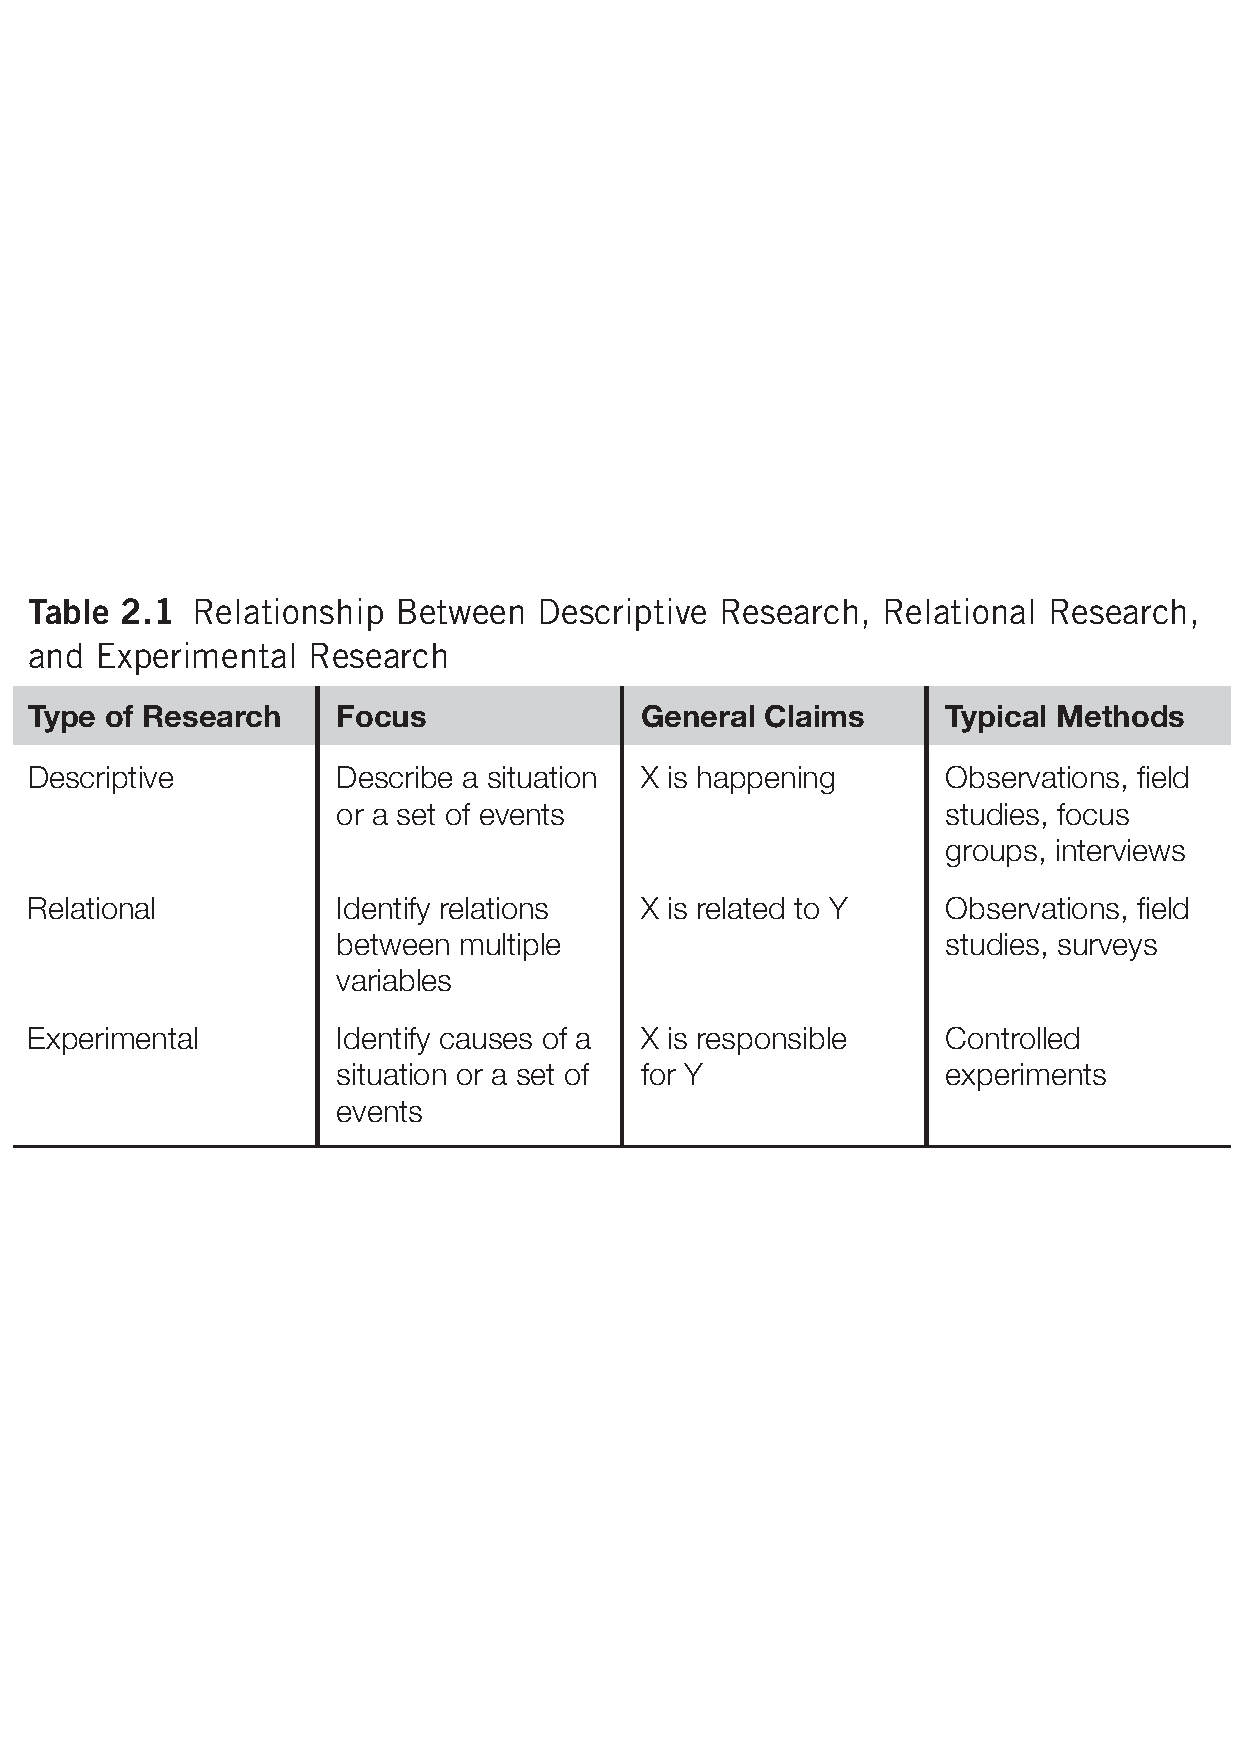
\includegraphics[scale=0.5]{img/Lazar-relationships-research.pdf}
    \end{figure}
   Lazar, J., Feng, J. H. and Hochheiser, H. (2017). Research Methods in Human-Computer Interaction. Morgan Kaufmann. \cite[p.27]{Lazar.et.al.2017.research}
\end{frame}
%
%
\begin{frame}
\frametitle{Quantitative Methods: ``How often?'' or ``How long?'' questions}
\begin{itemize}
\item \textbf{Experimental design} (chapter 2): development of research hypotheses and testing the validity. Null hypothesis vs\ alternative hypothesis, independent vs dependent variables, randomization. Between-group design (between groups) vs\ within-group design (repeated measures).
\begin{itemize}
\item Significance tests allow us to determine how confident we are that the results observed from the sampling population can be generalized to the entire population. For example, a test that is significant at $P<0.05$ suggests that we are confident that 95\% of the time the test result correctly applies to the entire population.
\item P-value: Probability value. The lower the value, the more unlikely that the null hypothesis is true. Depending on the result, we accept or reject the null hypothesis (determined by the significance level or threshold).
\end{itemize}
\item \textbf{Surveys}: a set of questions to which an individual is asked to respond. They are frequently used to describe populations and to explain behaviors. Considered one of the easiest methods. Typically broad but not deep.
\end{itemize}
\end{frame}
%
\begin{frame}
\frametitle{Qualitative Methods: ``Why?'' questions}
\begin{itemize}
\item \textbf{Diaries}: A document created by an individual who maintains regular recordings about events in their life, at the time that those events occur. See cultural probes by William Gaver \cite{Gaver.2004.cultural}.
\item \textbf{Case studies}: An in-depth study of a specific instance (or a small number of instances) within a specific real-life context. Close examination of individual cases can be used to build understanding, generate theories and hypotheses, present evidence for the existence of certain behavior, or to provide insight that would otherwise be difficult to gather.
\item \textbf{Interviews} (individuals) and \textbf{focus groups} (multiple users at once): Direct feedback from interested individuals. Deep but not broad.
\item \textbf{Ethnography}: A combination of observation, interviews, and participation. Ethnographic research projects use deep immersion and participation in a specific research context to develop an understanding that would not be achievable with other, more limited research approaches.
\end{itemize}
\end{frame}
%
\begin{frame}
\frametitle{Mixed Methods}
\begin{itemize}
\item Mixing of qualitative and quantitative data, methods, methodologies, and/or paradigms in a research study or set of related studies.
\begin{itemize}
\item \emph{Quantitatively driven approaches/designs} in which the research study is, at its core, a quantitative study with qualitative data/method added to supplement and improve the quantitative study.
\item \emph{Qualitatively driven approaches/designs} in which the research study is, at its core, a qualitative study with quantitative data/method added to supplement and improve the qualitative study.
\item \emph{Interactive or equal status designs} in which the research study equally emphasizes (interactively and through integration) quantitative and qualitative data, methods, methodologies, and paradigms. 
\end{itemize}
\end{itemize}
Creswell, J. W. and Creswell, J. D. (2017). Research Design: Qualitative, Quantitative, and Mixed Methods Approaches. Sage Publications. \cite{Creswell.2017.research}
\end{frame}
%
\begin{frame}
\frametitle{Data collection vs\ data analysis}
\begin{itemize}
\item Traditional data collection (users' replies, users' actions, audio recordings, video recordings, field notes).
\item Automated data collection indirectly from humans (e.g. key logging and web site logs).
\item Data collection directly from humans through sensors focused on the body (e.g. facial EMG and eye-tracking).
\item Online data collection (e.g. crowdsourcing and big data).
\item Qualitative analysis (transcription, manual annotation) vs\ quantitative data analysis (statistical analysis).
\end{itemize}
\end{frame}
%
\begin{frame}
\frametitle{Working with Human Participants / Subjects}
\begin{itemize}
\item Working with human subjects involves many challenges.
\item Finding the right subjects is often difficult and time consuming, especially for evaluation of systems designed for specific populations or situations.
\item Research ethics require that participants must be treated fairly and with respect.
\begin{itemize}
\item \emph{Informed consent}: a mechanism to inform participants about the nature of the study so they can make a meaningful decision as to whether or not they really want to be involved.
\item Check regulations at your institution / country where you are conducting the research (e.g. consent forms, data protection acts, etc).
\item Low- vs\ high-risk studies.
\item Plan ahead your study.
\end{itemize}
\end{itemize}
\end{frame}
%
\begin{frame}
\frametitle{Group discussion: ``From Mice to Men - 24 years of Evaluation in CHI''}
\begin{itemize}
\item Any surprises? 
\item Any limitations? 
\item Is the title accurate?
\end{itemize}
\end{frame}
%
%
\begin{frame}
\frametitle{Evaluation in CHI}
 \begin{figure}
	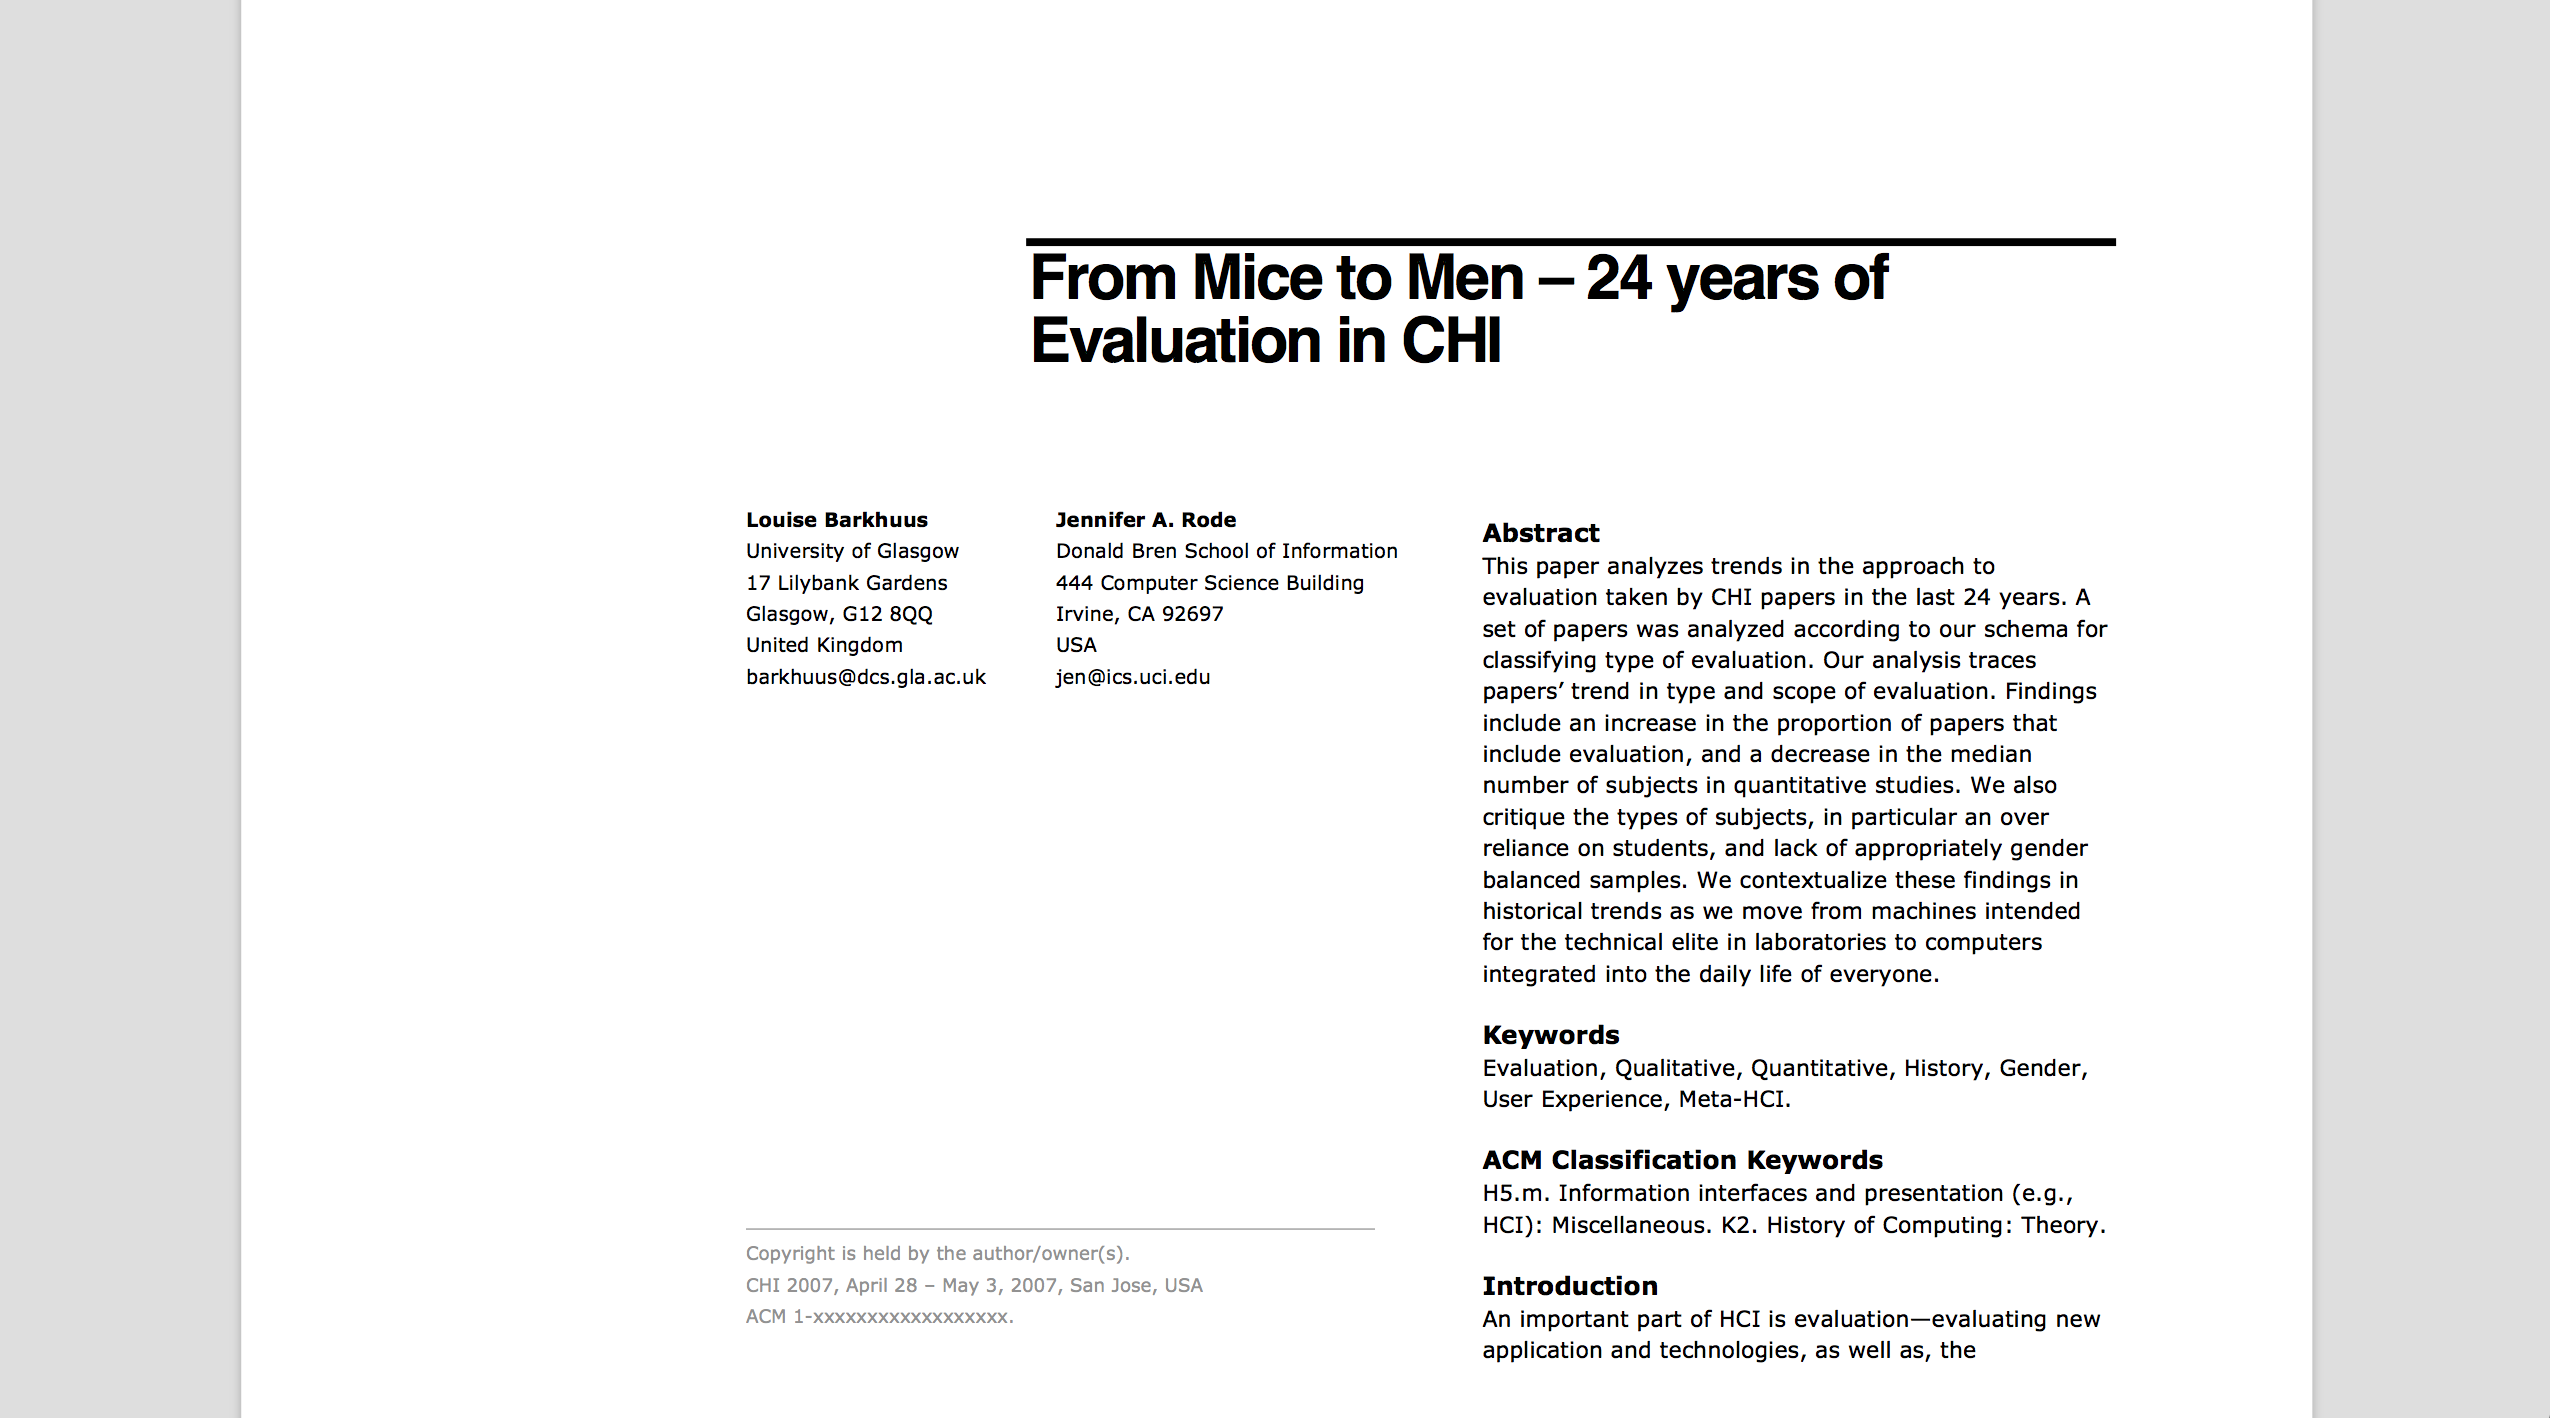
\includegraphics[scale=0.25]{img/Barkhuus-Rode-2007.png}\\
	\cite{Barkhuus.Rode.2007.evalchi}
    \end{figure}	
\end{frame}
%
\begin{frame}
\frametitle{}
\Huge{Human-Centered Design }
\end{frame}
%
\begin{frame}
\frametitle{The Human-Centered Design Process}
\begin{figure}
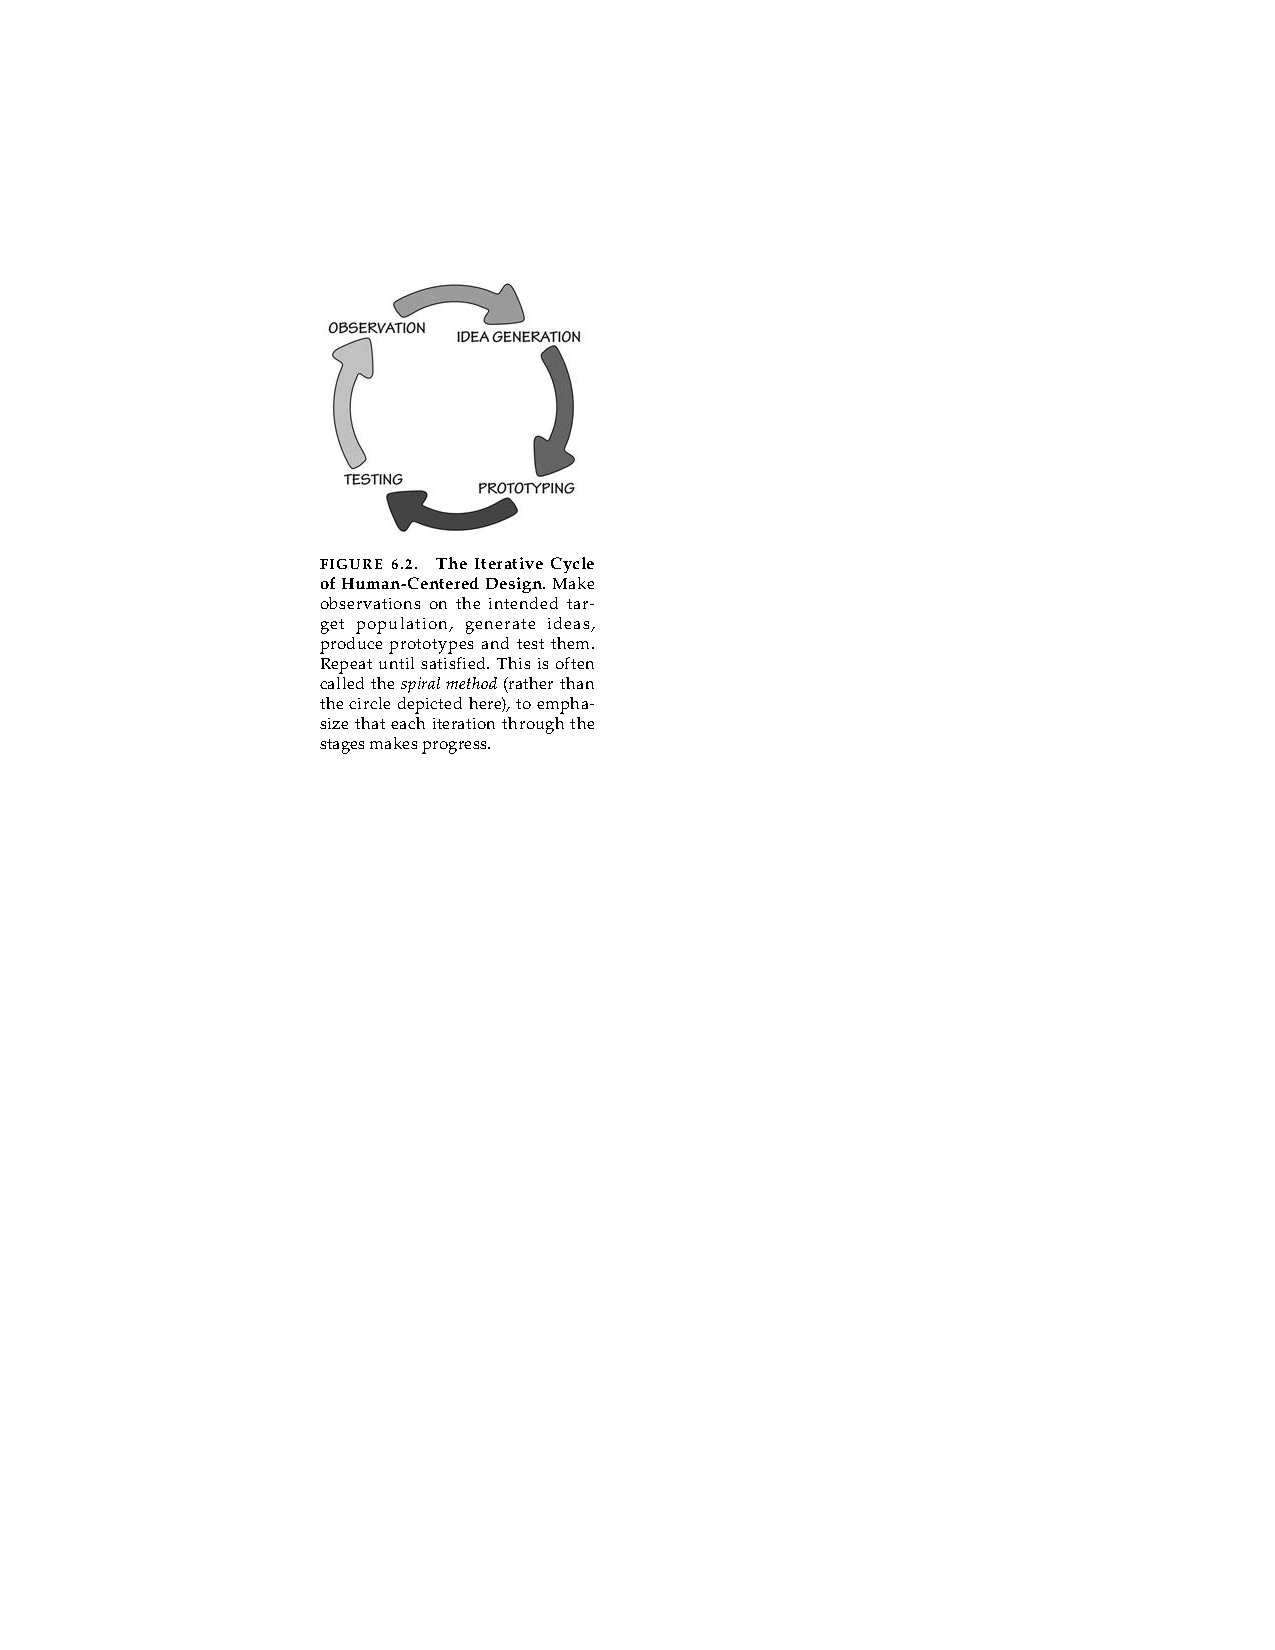
\includegraphics[scale=0.7]{img/Donald-Norman-human-centered-design.pdf}
\end{figure}
Norman, D. A. (2013/1988). \emph{The Design of Everyday Things}. Basic books. \cite{Norman.1988.psychology}
\end{frame}
%
\begin{frame}
\frametitle{The Human-Centered Design Process}
\begin{itemize}
\item \textbf{Observation}: The initial research to understand the nature of the problem itself. Design requirements are determined.
\item \textbf{Idea generation}: Generation of potential solutions. Generation of numerous ideas. Being creative without regard of constraints. Question everything.
\item \textbf{Prototyping}: Test the idea. Building of a quick prototype or mock-up of each potential solution. One popular technique is ``Wizard of Oz'' (mimic a powerful system), which is useful at early stages of development.
\item \textbf{Testing}: Gather a small group of people (similar to potential target population) and have them use the prototypes as nearly as possible to the way it is intended. Five people is generally a good number to start with (Jakob Nielsen).
\item \textbf{Iteration}: It enables continual refinement and enhancement. The goal is rapid prototyping and testing. ``Fail frequently, fail fast'' (David Kelly). 
\end{itemize}
{\scriptsize Norman, D. A. (2013/1988). \emph{The Design of Everyday Things}. Basic books. \cite{Norman.1988.psychology}}
\end{frame}
%
\begin{frame}
\frametitle{The Human-Centered Design Process}
\begin{quote}
Failures are to be encouraged---actually, they shouldn't be called failures: they should be thought of as learning experiences. If everything works perfectly, little is learned. Learning occurs when there are difficulties. \cite[p.229]{Norman.1988.psychology}\\
\vspace{5mm}
Norman, D. A. (2013/1988). \emph{The Design of Everyday Things}. Basic books.
\end{quote}
\end{frame}
%
\begin{frame}
\frametitle{The research and design cycle}
\begin{figure}
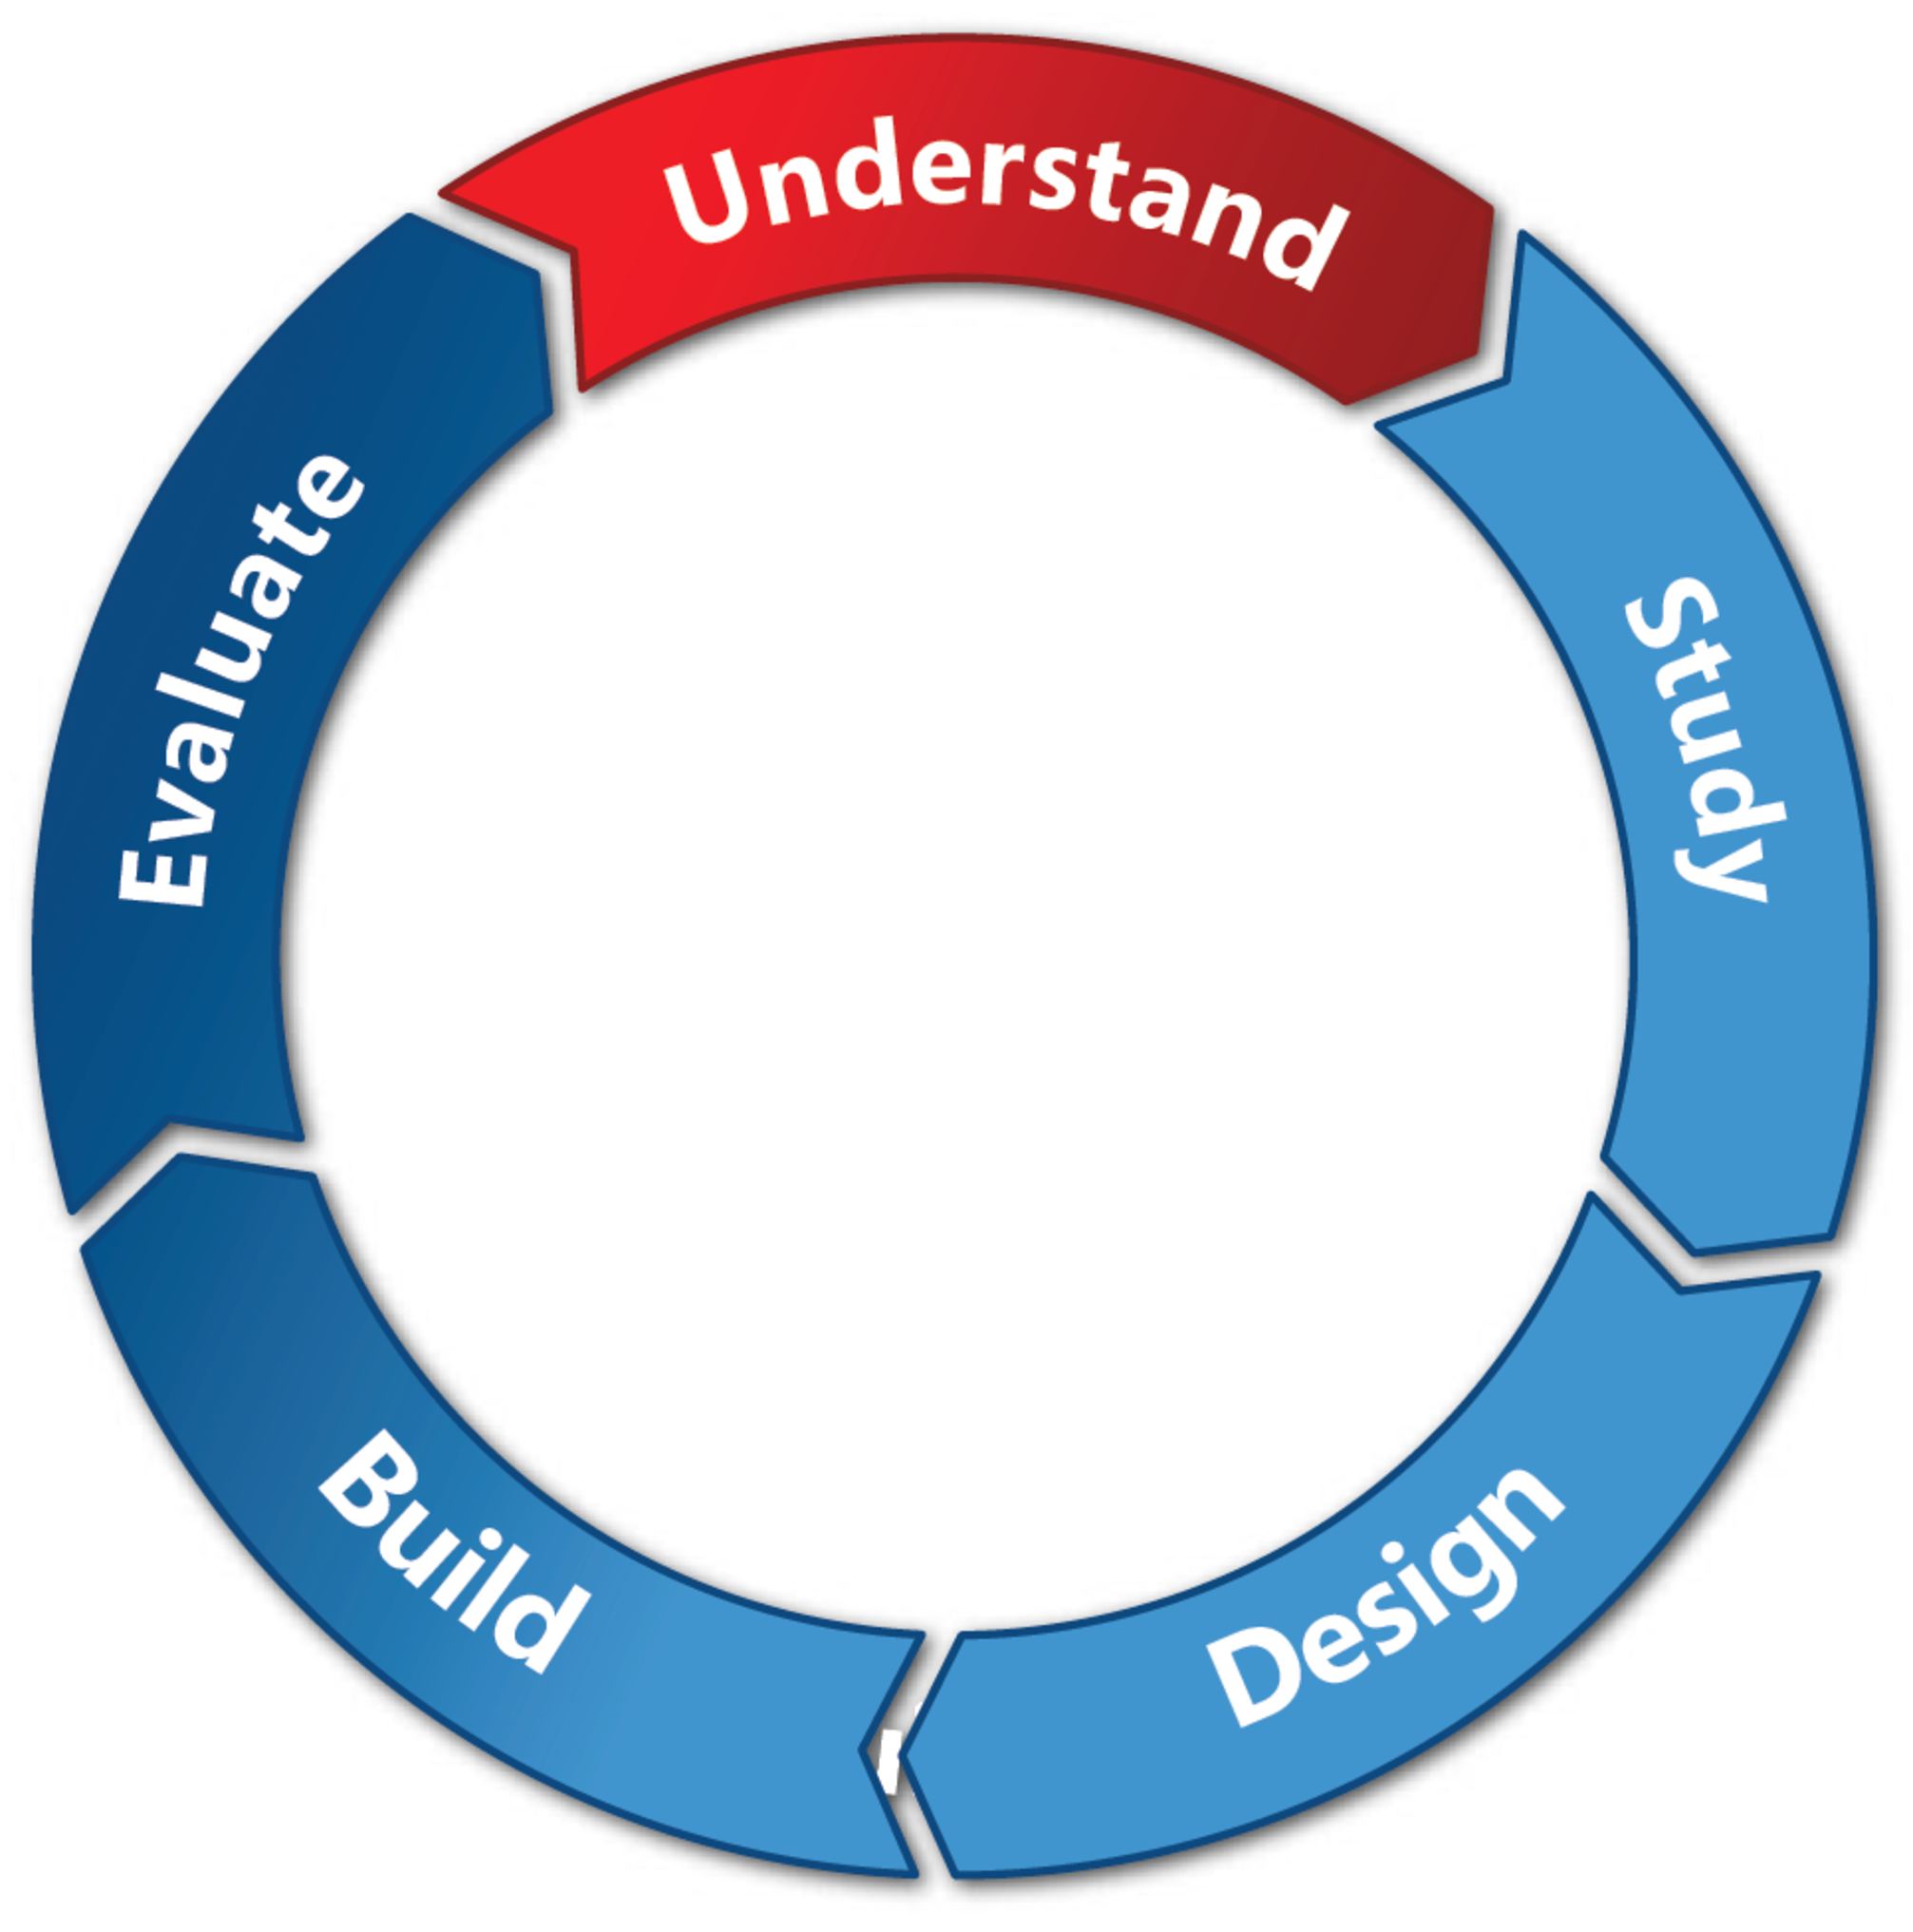
\includegraphics[scale=0.15]{img/design-cycle.pdf}
\caption{Extended user-centred, five-stage design/research model \cite{Harper.et.al.2008.being}}
\end{figure}
\end{frame}
%
\begin{frame}
\frametitle{Group discussion: How to evaluate your prototype borrowing HCI methods?}
What is your research question? What are potential ways of evaluating the music prototypes from the mini-hackathon of the Physical Computing Workshop considering quantitative, qualitative, and mixed research methods...
\begin{itemize}
\item Who would be your users? 
\item What are the challenges of your approach? 
\item What are the limitations of your approach? 
\end{itemize}
The teams summarize to the group their group discussion about the suitability of the research methods.
\end{frame}
%
\begin{frame}
\frametitle{Closing: What makes a good CHI paper?}
Discussion on Canvas: \url{https://uio.instructure.com/courses/22318/discussion_topics/58400}
\end{frame}
%
\begin{frame}
\frametitle{Human-Computer Interaction Day 2 - Group Assignment (post-class)}
\begin{itemize}
\item Send a summary (1 page max.)  of the *research methods* used in the selected article discussed in group during class on Tuesday 22 October 2019, from the CHI 2019 Best Papers (\url{https://chi2019.acm.org/2019/03/15/chi-2019-best-papers-honourable-mentions/}) before \textbf{Friday 25 October 2019 17:00}.  \\
This time you should focus on explaining the research methods used in terms of:
\begin{itemize} 
\item whether they are quantitative, qualitative, or mixed methods?
\item how are they related with the research question?
\item what are the limitations of this approach?
\item how do the authors address the limitations? 
\item what other research methods could have been used instead and why?
\end{itemize}
\item Assignment URL: \url{https://uio.instructure.com/courses/22318/assignments/28315}
\end{itemize}
\end{frame}
%
\begin{frame}[shrink=20]
  \frametitle{References}
  \printbibliography
\end{frame}
%
\end{document}
